% Note that the text in the [] brackets is the one that will
% appear in the table of contents, whilst the text in the {}
% brackets will appear in the main thesis.

%% CHAPTER HEADER /////////////////////////////////////////////////////////////////////////////////////
\chapter[Simulation Results and Model Validation]{Simulation Results and Model Validation}
\label{ch:validation}

%% CHAPTER INTRODUCTION ///////////////////////////////////////////////////////////////////////////////
The developed models require validation to assess the accuracy and reliability of the modelled physical processes.
Validation of the \ac{pzt} models is performed by analytical analysis of the electromechanical impedance of the circular sensor. 
On the other hand, the \ac{hsc} panel model is evaluated experimentally in two ways: by analysing the full wavefield obtained by the \ac{sldv} and by analysing the time signals measured by the \acp{pzt} setup.
%% INCLUDE SECTIONS ///////////////////////////////////////////////////////////////////////////////////
%% SECTION HEADER /////////////////////////////////////////////////////////////////////////////////////
\section{Validation of the \acs{pzt} model}
\label{sec:pztVal}

%% SECTION CONTENT ////////////////////////////////////////////////////////////////////////////////////
The current model, i.e. the curved boundary geometry approximated with the second-order elements, is validated by comparing the transducer impedance obtained by numerical simulation with (i) analytical model and (ii) experimental results.

The impedance Z is a ratio between voltage \((\Phi)\) and current \((I)\) defined as follows:
\begin{eqnarray}
	Z = \frac{\Phi}{I} = \frac{\Phi}{i\omega Q},
	\label{eq:impedance}
\end{eqnarray}
\nomtypeG[omega_ang]{\(\omega\)}{Angular frequency}{\(2\pi f_c\)}{\unit[per-mode = symbol]{\radian\per\second}}%
\nomtypeR[I]{\(I\)}{Electric current}{-}{\unit{\ampere}}%
\nomtypeD[i]{\(i\)}{Imaginary number}{\(sqrt{-1})\)}%
\nomtypeR[z_impedance]{\(Z\)}{Impedance}{\(\Phi/I\)}{\unit{\ohm}}%
where \(i=\sqrt{-1}\), \(\omega\) is the angular frequency.
In the case of numerical simulation, \(\Phi\) is assumed as the 1.5-cycle Hann windowed sine pulse at carrier frequency 150 \unit{\kHz}, and \(Q\) is the charge induced on the electrode calculated by Eq. (\ref{eq:pzt_sem}).
The excitation signal has significant values in the 0-300 \unit{\kHz} frequency range, as shown in Fig.~\ref{fig:impedance}(\textbf{a}).
The analytical model derived by Giurgiutiu \cite{giurgiutiu2009micromechatronics} is defined as:
\begin{eqnarray}
	Z = \frac{1}{i\omega C_0}\left[\left(1-k_p^2\right)+k_p^2\frac{u_r}{u_I}\right],
\end{eqnarray}
\nomtypeR[Capaci]{\(C_0\)}{Transducer free capacitance}{-}{\unit{\farad}}%
\nomtypeD[kp]{\(k_p\)}{Transducer planar coupling coefficient}{-}%
where \(C_0\) is the free capacitance of the sensor, \(k_p\) is the planar coupling coefficient, \(u_r\) is the displacement response, and \(u_I\) is the induced displacement.
Additionally, for comparison, the response of the \ac{sem} with curved boundary approximated by linear elements was included.
All models refer to the free transducer shown in Fig. \ref{fig:hioki}\textbf{(a)}, i.e. soldered wires and thin electrode coatings have been omitted.

\begin{figure}[H]
	\begin{center}
		\includegraphics[width=0.95\textwidth]{Chapter_6/hioki}
	\end{center}
	\caption{Setup to impedance measurement, \textbf{(a)} Hioki impedance analyser, \textbf{(b)} free \ac{pzt}, \textbf{(c)} transducer with soldered wires ready for measurements.}
	\label{fig:hioki}
\end{figure}
For experimental validation, an impedance analyzer (Hioki, IM 3570) was used to determine the electric current flowing through the transducer under the influence of applied voltage in the form of a sine signal with a variable frequency in the range of 1-300 \unit{\kHz}.
Both characteristics are used to determine the impedance according to Eq. \ref{eq:impedance}.
The measurements were taken at room temperature and averaged 50 times to improve the signal-to-noise ratio.

\begin{figure}[H]
	\begin{center}
		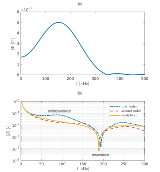
\includegraphics[width=0.95\textwidth]{Chapter_6/impedance}
	\end{center}
	\caption{Validation of the \acf{pzt} model (\textbf{a}) the frequency spectrum of the excitation signal, (\textbf{b}) impedance response of the transducer for numerical model with first order approximation of the boundary dash-dot line, numerical model with second order approximation of the curved boundary dashed line, analytical model dotted line and experimental measurements solid line.}
	\label{fig:impedance}
\end{figure}

It can be notice in Fig.~\ref{fig:impedance}(\textbf{b}) that the impedance of the model with second order approximation elements is in very good agreement with the analytical solution and to experimental results to the resonance peak.
The resonant peak occurred near 190 \unit{\kHz} for second order model and analytical one and 194 \unit{\kHz} in case of experimental measurement.
The model with a first-order approximation is a better fit for the experiment in frequencies above the resonant peak.
In addition, an additional antiresonance peak occurred around 90 \unit{\kHz}, which was not observed in the previous two models and experimental result.

The discrepancy in impedance based on the models and experiment may be due to uncontrolled ambient condition during the measurements and accuracy of piezo and electromechanical properties provided by the manufacturer. 
Additionally, the models were simplified by excluding the wires and solder unlike the tested transducer shown in Fig. \ref{fig:hioki}\textbf{(b)}.


%% SECTION HEADER /////////////////////////////////////////////////////////////////////////////////////
\section{Experimental Setup Configuration}
\label{sec:setup}

%% SECTION CONTENT ////////////////////////////////////////////////////////////////////////////////////

The presented model was validated with results from two experimental studies.
The first one was performed for determination of the full wavefield of the propagating waves by the \ac{sldv} (Polytec PSV–400).
The second study was performed for wave acquisition by the \ac{pzt} sensor.
The schematic of the experimental setup is shown in Figure~\ref{fig:setup}.
The sample of interest was a not-regular hexagonal aluminium honeycomb bonded to one \ac{cfrp} plate  using the epoxy adhesive (Loctite EA3479B) as shown in Figure~\ref{fig:honeycomb}(\textbf{a}).%PF: label acc. to figure caption.
The subject of the parametric study was the effect of the disbond size on the propagating GW.

\begin{figure}[H]
	%	\begin{center}
	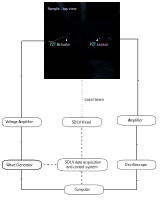
\includegraphics[width=1\linewidth]{Chapter_6/setup}
	%	\end{center}
	\caption{Experimental setup for the (1) \ac{sldv} measurement---dashed line and (2) PZT wave acquisition---solid line.}
	\label{fig:setup}
\end{figure}
\vspace{-12pt}
\begin{figure}[H]
	%	\begin{center}
	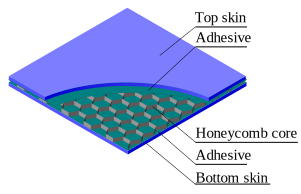
\includegraphics[width=1\linewidth]{Chapter_6/honeycomb}
	%	\end{center}
	\caption{Sample configuration: (\textbf{a}) top view of the sample, (\textbf{b}) honeycomb sandwich substructures and (\textbf{c}) details of the honeycomb cell.}
	\label{fig:honeycomb}
\end{figure}


After a reference measurement was made on an intact sample, several measurements were taken for the subsequent damage introduced on the same specimen.
The circular area of the core was detached from the adhesive at the center of the plate using a sharp hooked tool.
For this purpose, the bottom skin was omitted so that damage could be introduced.
The damage size was controlled by its diameter \(\Phi_D=\left [10, 30, 50, 70, 90, 110, 130 \right ]\) mm.

The generation and reception of elastic waves were achieved with a pair of \ac{pzt} transducers mounted on the skin top surface with the cyanoacrylate glue.
The coordinates of the actuator were \((x_1,y_1)=(-100,0)\) mm,	and for the sensor, \((x_2,y_2)=(100,0)\) mm.
The dimensions of the sample components were as follows:
\begin{itemize}
	\item \ac{cfrp} skin: \(L \times W \times H = 500 \times 500\ \times 1.5\) mm,
	\item Aluminium core: \(g=14.5\) mm, \(w=0.1\) mm, \(h_1=11\) mm, \(h_2=5\) mm, \(l_1=10.4\) mm, \(l_2=6\) mm,
	\item Epoxy adhesive: \(L\times W \times H = 500 \times 500 \times 0.3\) mm,
	\item NCE51 \ac{pzt}: \(\Phi_{PZT}=10\) mm, \(h=0.5\) mm,
	\item Cyanoacrylate glue: \(\Phi_{CG}=10\) mm, \(h=0.05\) mm.
\end{itemize}

The \(N_c=5\) cycle Hann windowed signal at carrier frequencies \mbox{\(f_c=[75,100,125,150]\) kHz} was generated using an arbitrary waveform generator (National Instruments, PXI 5413).
The signal was amplified 40 times and supplied to the \ac{pzt} actuator (Noliac, NCE51).
Each measurement was conducted in the room temperature and averaged 20~times in order to improve the signal to noise ratio.
%% SECTION HEADER /////////////////////////////////////////////////////////////////////////////////////
\section{Results of \acl{hsc} validation with the \acl{sldv} setup}
\label{sec:resuls_sldv}
%% SECTION CONTENT ////////////////////////////////////////////////////////////////////////////////////
Figures~\ref{fig:fullfield_50_0}, \ref{fig:fullfield_100_0} and \ref{fig:fullfield_150_0} present the full wavefield in the healthy sample.
The experimental measurements and the \ac{fcgm} snapshots show that the wavefront distortion is rising with the frequency.
Because the wavelength decreases as the frequency increases, a higher frequency signal is more likely to induce wave reflections from the core walls.
This effect can not be observed in the case of the \ac{hcgm}.

\begin{figure}[!hbt]
	\begin{center}
		\includegraphics[width=0.95\textwidth]{Chapter_6/fullfield_50_0}
	\end{center}
	\caption{The top surface out-of-plane velocity snapshots for (\textbf{a}) the \acf{fcgm}, (\textbf{b}) the experimental results obtained by \acf{sldv}, and (\textbf{c}) the \acf{hcgm} in the \textbf{healthy~sample at 50 kHz}}
	\label{fig:fullfield_50_0}
\end{figure}
\begin{figure}[!hbt]
	\begin{center}
		\includegraphics[width=0.95\textwidth]{Chapter_6/fullfield_100_0}
	\end{center}
	\caption{The top surface out-of-plane velocity snapshots for (\textbf{a}) the \acf{fcgm}, (\textbf{b}) the experimental results obtained by the \acf{sldv}, and (\textbf{c}) the \acf{hcgm} in the \textbf{healthy~sample at 100 kHz}}
	\label{fig:fullfield_100_0}
\end{figure}
\begin{figure}[!hbt]
	\begin{center}
		\includegraphics[width=0.95\textwidth]{Chapter_6/fullfield_150_0}
	\end{center}
	\caption{The top surface out-of-plane velocity snapshots for (\textbf{a}) the \acf{fcgm}, (\textbf{b}) the experimental results obtained by the \acf{sldv}, and (\textbf{c}) the \acf{hcgm} in the \textbf{healthy~sample at 150 kHz}}
	\label{fig:fullfield_150_0}
\end{figure}

In case of the damaged sample, the wavefront was not distorted in the damage area bounded by dashed white rectangle in Figures~\ref{fig:fullfield_50_5}, \ref{fig:fullfield_100_5} and \ref{fig:fullfield_150_5} for all three cases.
Due to the lack of wave leakage into the core, the wave propagated smoothly through the skin.
For the experimental sample and the \ac{fcgm}, interference of waves reflected from the cells and the damage boundary is observed.
The wave interference observed in the \ac{hcgm} refers to waves reflected only from the defect.

\begin{figure}[!hbt]
	\begin{center}
		\includegraphics[width=0.95\textwidth]{Chapter_6/fullfield_50_5}
	\end{center}
	\caption{The top surface out-of-plane particle velocity snapshots for (\textbf{a}) the \acf{fcgm}, (\textbf{b}) the experimental results obtained by the \acf{sldv}, and (\textbf{c}) the \acf{hcgm} \textbf{with removed core elements at 50 kHz} in damaged area for both numerical models}
	\label{fig:fullfield_50_5}
\end{figure}
\begin{figure}[!hbt]
	\begin{center}
		\includegraphics[width=0.95\textwidth]{Chapter_6/fullfield_100_5}
	\end{center}
	\caption{The top surface out-of-plane velocity snapshots for (\textbf{a}) the \acf{fcgm}, (\textbf{b}) the experimental results obtained by the \acf{sldv}, and (\textbf{c}) the \acf{hcgm} \textbf{with removed core elements at 100 kHz} in damaged area for both numerical models}
	\label{fig:fullfield_100_5}
\end{figure}
\begin{figure}[!hbt]
	\begin{center}
		\includegraphics[width=0.95\textwidth]{Chapter_6/fullfield_150_5}
	\end{center}
	\caption{The top surface out-of-plane velocity snapshots for (\textbf{a}) the \acf{fcgm}, (\textbf{b}) the experimental results obtained by the \acf{sldv}, and (\textbf{c}) the \acf{hcgm} \textbf{with removed core elements at 150 kHz} in damaged area for both numerical models}
	\label{fig:fullfield_150_5}
\end{figure}
\clearpage
%% SECTION HEADER /////////////////////////////////////////////////////////////////////////////////////
\section{Results of \acl{hsc} validation with \aclp{pzt} wave acquisition setup}
\label{sec:resuls_pzt}
%% SECTION CONTENT ////////////////////////////////////////////////////////////////////////////////////
Validation of the honeycomb structure models and a separate \ac{cfrp} plate intended for \ac{hsc} sample were done by comparing the group velocity and amplitude of the first packet of \ac{s0} and \ac{a0} arriving at the sensor.
Figure~\ref{fig:signal_exp_raw} contains examples of the experimentally obtained raw signals for the healthy and damaged samples.
The raw signals were processed for noise reduction and next an envelope of the signals was calculated.
The envelope was used to obtain the amplitude and group velocity of the mods for the model validation and was used in the analytical assessment of damage magnitude.
\begin{figure}[!htb]
	\begin{center}
		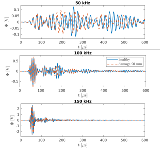
\includegraphics[width=0.95\textwidth]{Chapter_6/signal_exp_raw}
	\end{center}
	\caption{Raw signals registered by the sensor in \acl{hsc} for the specimen at healthy (solid line) and the damaged state - disbonds width of 90 \unit{\mm} (dashed line)}
	\label{fig:signal_exp_raw}
\end{figure}
\pagebreak

Signal processing followed the diagram shown in Figure~\ref{fig:signal_processing}.
A preliminary step was a conversion of the signals from the time domain to the frequency domain by the \ac{fft}.
Then, the band-pass filter was applied in the range \(0.5f_c-1.5f_c\).
For this purpose a Butterworth filter of 20th order was used.
After filtering, the signal was converted back to the time domain by the \ac{ifft}.
Lastly, the envelope of the signal \(e(t)\) was obtained using Eq. (\ref{eq:envelope}).

\begin{figure}[!htb]
	\begin{center}
		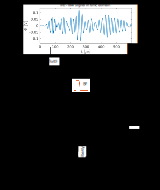
\includegraphics[width=0.95\textwidth]{Chapter_6/signal_processing}
	\end{center}
	\caption{Raw signals registered by the sensor in \acl{hsc} for healthy state and damage of 90 \unit{\mm} width}
	\label{fig:signal_processing}
\end{figure}

The group velocity was derived from the signal envelope related to particular Lamb wave mode and its \ac{tof}.
The \ac{tof} is a difference between the arrival of the maximum amplitude of the envelope of considered mode at the sensor \((\mathrm{T}_1)\) and the half time of the excitation pulse \(\left(\mathrm{T}_0=0.5/f_m\right)\).
Since the distance between the transducers was constant \(l=200\) \unit{\mm}, the group velocity equals
\begin{eqnarray}
	C_g = \frac{\mathrm{ToF}}{l}=\frac{T_1-T_0}{l}.
\end{eqnarray}

The signal envelopes are shown in Figure~\ref{fig:single_skin} for single \ac{cfrp} plate, Figure~\ref{fig:hsc_full} for the \ac{fcgm}, and Figure~\ref{fig:hsc_homo}, from which the velocities and amplitudes of the wave mods were determined.
\begin{figure}[!htb]
	\begin{center}
		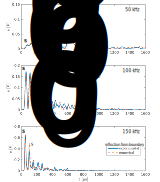
\includegraphics[width=0.95\textwidth]{Chapter_6/single_skin}
	\end{center}
	\caption{The signal envelope for single \acs{cfrp} skin; experimental vs. numerical simulation}
	\label{fig:single_skin}
\end{figure}

For the single \ac{cfrp} plate, Table~\ref{tab:group_velocity_cfrp} gives the determined velocities and amplitudes of the modes together with the percentage errors defined by
\begin{eqnarray}
	\delta = \left|\frac{x^{num}-x^{exp}}{x^{exp}}\right|\times100\%,
	\label{eq:perc_err}
	\nomtypeG[delta]{\(\delta\)}{Percentage error}{}{\%}%
\end{eqnarray}
where \(x^{num}\) and \(x^{exp}\) are the numerical and experimental values, respectively.
It can be noticed that the model is in good agreement with experimental results.
All values are within an error of up to 10\%, except for the \ac{s0} and \ac{a0} amplitudes for 50 and 100 \unit{\kHz}, respectively.
For these cases, the error is about 25\%.
The \ac{a0} mode at 150 \unit{\kHz} in Figure~\ref{fig:hsc_homo} was not identified because the high amplitude \ac{s0} reflections mask it.

Regarding \ac{hsc} panel, the best results were achieved for the \ac{fcgm} as it is shown in Table~\ref{tab:group_velocity_hsc}.
The velocity error is less than 10\% for both modes except for the signal at 50 \unit{\kHz}. 
In the case of signals amplitude, the simulation results are underestimated.
Only the \ac{s0} at 100 and 150 \unit{\kHz} has the error less than 15\%.
For the \ac{hcgm}, the best result were obtained for the \ac{s0} at 150 \unit{\kHz} with error less than 11\%.
Amplitudes of the \ac{a0} for this model are more accurate than the \ac{fcgm} with the errors below 15\%.
\begin{figure}[!htb]
	\begin{center}
		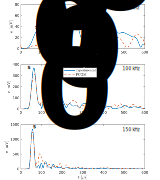
\includegraphics[width=0.95\textwidth]{Chapter_6/HSC_full}
	\end{center}
	\caption{The signal envelope for the \acl{hsc} structure; experimental vs. the \acf{fcgm}}
	\label{fig:hsc_full}
\end{figure}

\begin{figure}[!htb]
	\begin{center}
		\includegraphics[width=0.95\textwidth]{Chapter_6/HSC_homo}
	\end{center}
	\caption{The signal envelope for the \acl{hsc} structure; experimental vs. the \acf{hcgm}}
	\label{fig:hsc_homo}
\end{figure}
\begin{table}[!htb]
	\small
	\tabcolsep=0.2cm
	\centering
	\caption{\label{tab:group_velocity_cfrp} Comparison between amplitudes and group velocities obtained from the simulations and experiments for the single \acs{cfrp} plate}
	\begin{tabular}{cccccccc}
		\toprule
		& & \multicolumn{3}{c}{\(C_g\)} & \multicolumn{3}{c}{Amp.}\\
		Mode & Frequency & Exp. & Num. & \(\delta\)& Exp. & Num. & \(\delta\)\\
		& \unit{\kHz} & \unit[per-mode = symbol]{\m\per\s} & \unit[per-mode = symbol]{\m\per\s} & \% & \unit{\mV} & \unit{\mV} & \% \\
		\midrule
		\multirow{3}{*}{\ac{s0}} & 50 & 6079 & 5865 & \textcolor{green}{3.52}& 12 & 171 & \textcolor{red}{25.0} \\
		&100& 5571 & 5747 & \textcolor{green}{3.16} & 171 & 162 & \textcolor{green}{5.26}\\
		&150& 5764 & 5698 & \textcolor{green}{1.15} & 648 & 664 & \textcolor{green}{2.47}\\
		\midrule
		\multirow{3}{*}{\ac{a0}} &50& 1341 & 1325 & \textcolor{green}{0.74} & 134 & 125 & \textcolor{green}{6.72}\\
		&100& 1550 & 1396 & \textcolor{green}{9.74} & 84 & 104 & \textcolor{red}{23.8}\\
		\bottomrule
	\end{tabular}
\end{table}

Errors in the models may be due to several factors.
The most important ones include differences in material properties of used components.
In the models, an average thickness of the adhesive layer was assumed; obtaining precise thickness of the adhesive layer in the specimen preparation is difficult under workshop conditions.
The models also assumed the same shape for each core cell, whereas in practice, the geometry was different because of in-plane deformation of the core during the sample preparation.
The velocity in the panel varies with the angle of propagation due to anisotropy of \ac{cfrp} plate and the geometry of the honeycomb core.
In the models, the direction of wave propagation between the sensors was assumed to coincide with the skin and core orientation.
\clearpage


\begin{table}[!htb]
	\small
	\tabcolsep=0.15cm
	\centering
	\caption{\label{tab:group_velocity_hsc} Comparison between amplitudes and group velocities obtained from the simulations based on the \acf{fcgm} and the \acf{hcgm} and experiments for \acl{hsc}}
	\begin{tabular}{cccccccccccc}
		\toprule
		& & \multicolumn{5}{c}{\(C_g\)} & \multicolumn{5}{c}{Amp.}\\
		Mode & Freq.& Exp. & \ac{fcgm} & \(\delta\) & \ac{hcgm} & \(\delta\) &  Exp. & \ac{fcgm} & \(\delta\) & \ac{hcgm} & \(\delta\)\\
		& \unit{\kHz} & \unit[per-mode = symbol]{\m\per\s} & \unit[per-mode = symbol]{\m\per\s} & \% & \unit[per-mode = symbol]{\m\per\s} & \% & \unit{\mV} & \unit{\mV} & \%& \unit{\mV} & \% \\
		\midrule
		\multirow{3}{*}{\ac{s0}} & 50 & 6452 & 8696 & {34.78} & 8333 & {29.15} & 32 & 6 & \textcolor{red}{81.25} & 3 & \textcolor{red}{90.63}\\
		&100& 5263 & 5128 & \textcolor{green}{2.57} & 5714 & \textcolor{green}{8.57} & 369 & 314 & \textcolor{green}{14.91} & 138 & \textcolor{red}{62.6}\\
		&150& 5085 & 5217 & \textcolor{green}{2.60} & 4959 & \textcolor{green}{2.48} & 1341 & 1239 & \textcolor{green}{7.61} & 1482 & \textcolor{green}{10.51}\\
		\midrule
		\multirow{3}{*}{\ac{a0}} & 50 & 966 & 926 & \textcolor{green}{4.14} & 1316 & {36.23} & 62 & 76 & {22.58} & 63 & \textcolor{green}{1.61}\\
		& 100 & 2174 & 2151 & \textcolor{green}{1.06} & 2273 & \textcolor{green}{4.55} & 137 & 179 & {30.66} & 117 & \textcolor{green}{14.60}\\
		\bottomrule
	\end{tabular}
\end{table}

\section{Conclusions}
\label{sec:conclusionsValid}

%% SECTION CONTENT ////////////////////////////////////////////////////////////////////////////////////
In this chapter, I presented the experimental validation of the \ac{fcgm} and \ac{hcgm}.
It is shown that the \ac{fcgm} better expresses the wave propagation in the \ac{hsc} than the simplified model.
The snapshots of the full wavefield showed wave interference in the core cells, which is impossible to obtain in the \ac{hcgm}.
The full-field analysis also showed a lack of wave leakage into the core at the damaged area.
This phenomenon will be the basis for determining the effect of the damage on wave propagation.
The velocity of the wave propagation for both models is in good agreement with the \ac{pzt} measurements.